\documentclass[11pt,psfig]{article}
\usepackage{epsfig}
\usepackage{times}
\usepackage{amssymb}
\usepackage{float}

\newcount\refno\refno=1
\def\ref{\the\refno \global\advance\refno by 1}
\def\ux{\underline{x}}
\def\uw{\underline{w}}
\def\bw{\underline{w}}
\def\ut{\underline{\theta}}
\def\umu{\underline{\mu}} 
\def\bmu{\underline{\mu}} 
\def\be{p_e^*}
\newcount\eqnumber\eqnumber=1
\def\eq{\the \eqnumber \global\advance\eqnumber by 1}
\def\eqs{\eq}
\def\eqn{\eqno(\eq)}

 \pagestyle{empty}
\def\baselinestretch{1.1}
\topmargin1in \headsep0.3in
\topmargin0in \oddsidemargin0in \textwidth6.5in \textheight8.5in
\begin{document}
\setlength{\parskip}{1.2ex plus0.3ex minus 0.3ex}


\thispagestyle{empty} \pagestyle{myheadings} \markright{Homework
1: CS 216, Image Understanding: Spring 2014}



\title{CS 216 Homework 1}
\author{Zachary DeStefano, 15247592}
\date{Due Date: April 9}

\maketitle

\vfill\eject

\section*{Problem 4}

\subsection*{Problem 4a}

The variable $x$ will be assigned to an array that is the numbers 1 through 5 arranged in a random order. 

\subsection*{Problem 4b}

The variable $a$ will be assigned to an array that is the numbers 1 through 10 arranged in chronological order. The variable $b$ will end up being assigned an array that is the numbers $1,4,7,10$ because it is the first number and then every third number after that. 

\subsection*{Problem 4c}

The variable $f$ will be assigned to an array that is the numbers 1501 to 2000 in chronological order. The variable $g$ will be assigned to the indices of $f$ where the entries are greater than $1850$ which is $351$ to $500$. The variable $h$ will then be assigned an array that is the numbers $1851$ to $2000$.  

\subsection*{Problem 4d}

The variables $x$ will be assigned to a vector of 10 entries where each entry has value 22. The variable $y$ will be assigned the sum of the entries which will be 220.

\subsection*{Problem 4e}

The variable $a$ will be assigned an array that is the numbers 1 to 1000 in chronological order. The variable $b$ will be assigned a vector that is the numbers 1 to 1000 in reverse order. 

%\begin{figure}[H]
%\centering
%\includegraphics[height=4in]{prob1plot.jpg}
%\caption{Probability of Class Labels with decision boundaries marked}
%\end{figure}

\section*{Problem 5}

\begin{figure}[H]
\centering
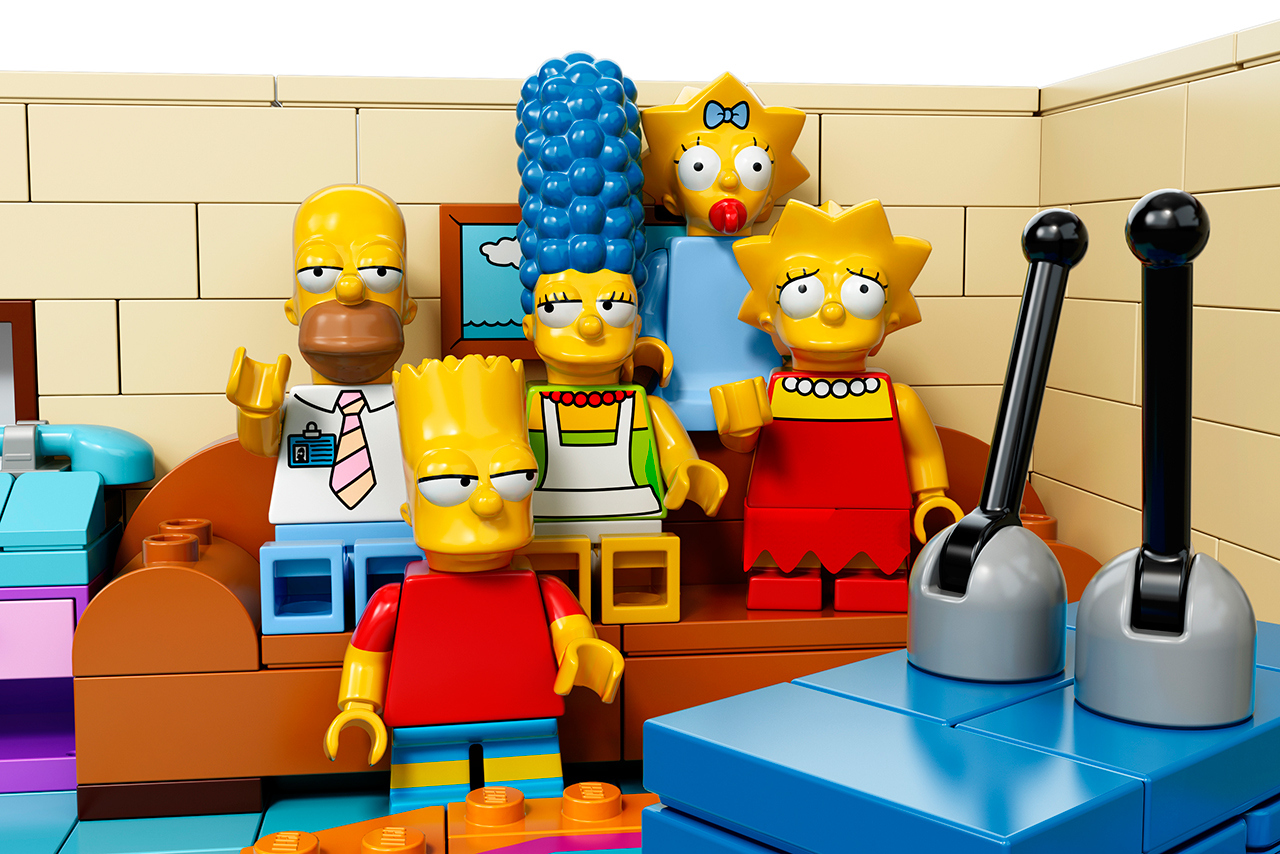
\includegraphics[height=4in]{originalImageProb5.jpg}
\caption{Original Image from the Internet}
\end{figure}

\begin{figure}[H]
\centering
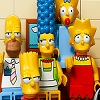
\includegraphics[height=1in]{modifiedImageProb5.jpg}
\caption{Modified 100 by 100 image}
\end{figure}

\begin{figure}[H]
\centering
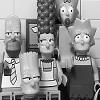
\includegraphics[height=1in]{blackWhiteImage.jpg}
\caption{Modified 100 by 100 image in grayscale}
\end{figure}

Here is the initialization code:

\begin{verbatim}

A = rgb2gray(imread('modifiedImageProb5.jpg'));
A = im2double(A);
imwrite(A,'blackWhiteImage.jpg','JPEG');

\end{verbatim}

\subsection*{Problem 5a}

\begin{figure}[H]
\centering
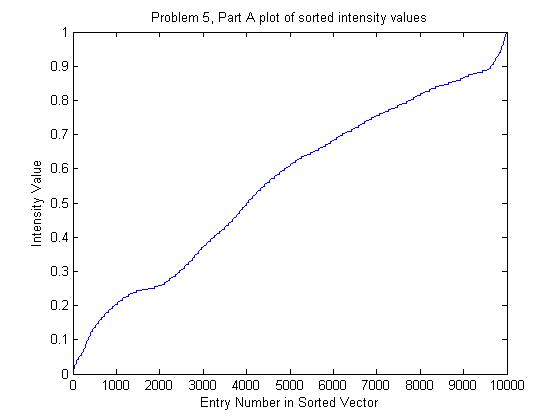
\includegraphics[height=2in]{prob5partAplot.jpg}
\caption{Plot of Intensity Values}
\end{figure}

Here is the code used to get the plot:

\begin{verbatim}

singleVectorA = A(:);
sortedValuesA = sort(singleVectorA);
figure
plot(sortedValuesA);
xlabel('Entry Number in Sorted Vector');
ylabel('Intensity Value');
title('Problem 5, Part A plot of sorted intensity values');

\end{verbatim}

\subsection*{Problem 5b}

\begin{figure}[H]
\centering
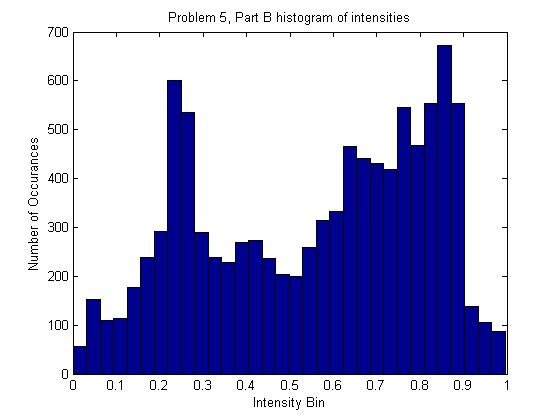
\includegraphics[height=2in]{prob5partBplot.jpg}
\caption{Histogram of Intensities with 32 bins}
\end{figure}

Here is the code used to get the plot:

\begin{verbatim}

figure
hist(singleVectorA,32);
xlabel('Intensity Bin');
ylabel('Number of Occurances');
title('Problem 5, Part B histogram of intensities');

\end{verbatim}

\subsection*{Problem 5c}

\begin{figure}[H]
\centering
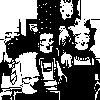
\includegraphics[height=1in]{partCimage.jpg}
\caption{Binary Image using 0.65 as the threshold}
\end{figure}

Here is the code used to get the image:

\begin{verbatim}

threshold = 0.65;
binaryA = zeros(size(A));
binaryA(A > threshold) = 1;
imwrite(binaryA,'partCimage.jpg','JPEG');

\end{verbatim}

\subsection*{Problem 5d}

\begin{figure}[H]
\centering
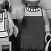
\includegraphics[height=0.5in]{partDimage.jpg}
\caption{Bottom Right Quadrant of A}
\end{figure}

Here is the code used to get the image:

\begin{verbatim}

sizeA = size(A);
sizeAhoriz = sizeA(1);
sizeAvert = sizeA(2);
bottomRightA = A(sizeAhoriz/2:sizeAhoriz,sizeAvert/2:sizeAvert);
imwrite(bottomRightA,'partDimage.jpg','JPEG');

\end{verbatim}

\subsection*{Problem 5e}

\begin{figure}[H]
\centering
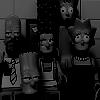
\includegraphics[height=1in]{partEimage.jpg}
\caption{New image with mean subtracted}
\end{figure}

Here is the code used to get the image:

\begin{verbatim}

meanBrightness = mean(singleVectorA);
meanSubtractedA = A-meanBrightness;
meanSubtractedA( meanSubtractedA < 0) = 0;
imwrite(meanSubtractedA,'partEimage.jpg','JPEG');

\end{verbatim}

\subsection*{Problem 5f}

\begin{verbatim}

function [ result ] = diceRoll_partF()
%DICEROLL_PARTF Summary of this function goes here
%   Detailed explanation goes here

result = floor(rand(1)*6) + 1;

end

\end{verbatim}

\subsection*{Problem 5g}

\begin{verbatim}

y = [1:6];
z = reshape(y,3,2);

\end{verbatim}

\subsection*{Problem 5h}

Result is that $x=0$ and $[r,c]=[95,99]$. Code to accomplish it is the following

\begin{verbatim}

x = min(singleVectorA);
[r,c] = find(A==x,1);

\end{verbatim}

\subsection*{Problem 5i}

The result is 5 unique values. Here is the code that was used:

\begin{verbatim}

v = [1 8 8 2 1 3 9 8];
sizeUniqueV = size(unique(v));
numUnique = sizeUniqueV(2);

\end{verbatim}

\subsection*{Problem 5 Compiled Code}

Here is the entire script used for problem 5, except for part F which was a separate function. This just puts all the code pieces from the previous sections together:

\begin{verbatim}

A = rgb2gray(imread('modifiedImageProb5.jpg'));
A = im2double(A);
imwrite(A,'blackWhiteImage.jpg','JPEG');

%Part A
singleVectorA = A(:);
sortedValuesA = sort(singleVectorA);
figure
plot(sortedValuesA);
xlabel('Entry Number in Sorted Vector');
ylabel('Intensity Value');
title('Problem 5, Part A plot of sorted intensity values');

%Part B
figure
hist(singleVectorA,32);
xlabel('Intensity Bin');
ylabel('Number of Occurances');
title('Problem 5, Part B histogram of intensities');

%Part C
threshold = 0.65;
binaryA = zeros(size(A));
binaryA(A > threshold) = 1;
imwrite(binaryA,'partCimage.jpg','JPEG');

%Part D
sizeA = size(A);
sizeAhoriz = sizeA(1);
sizeAvert = sizeA(2);
bottomRightA = A(sizeAhoriz/2:sizeAhoriz,sizeAvert/2:sizeAvert);
imwrite(bottomRightA,'partDimage.jpg','JPEG');

%Part E
meanBrightness = mean(singleVectorA);
meanSubtractedA = A-meanBrightness;
meanSubtractedA( meanSubtractedA < 0) = 0;
imwrite(meanSubtractedA,'partEimage.jpg','JPEG');

%diceRoll_partF.m is part F

%Part G
y = [1:6];
z = reshape(y,3,2);

%Part H
x = min(singleVectorA);
[r,c] = find(A==x,1);

%Part I
v = [1 8 8 2 1 3 9 8];
sizeUniqueV = size(unique(v));
numUnique = sizeUniqueV(2);

\end{verbatim}

\section*{Problem 6}

\subsection*{Helper method for getting image data}

The following function is used by the rest of the functions to get image data:

\begin{verbatim}

function [ colorImages, grayscaleImages ] = getImageSetData( dirname, fileformat )
%GETIMAGESETDATA This gets the multi-dimensional array of color image data
%                and grayscale image data. All images must be same size
%   Input
%       dirname: name of directory to search
%       fileformat: file format string for images to put into set
%   Output
%       colorImages: color data array
%       grayscaleImages: grayscale data array

dirString = strcat(dirname,fileformat);
setList = dir(dirString);
numImages = length(setList);
imnameStart = strcat(dirname,'/');

%get info on first image
firstColorImage = imread([imnameStart setList(1).name]);
firstGrayscaleImage = rgb2gray(firstColorImage);
colorImages = zeros([size(firstColorImage) numImages]);
grayscaleImages = zeros([size(firstGrayscaleImage) numImages]);

for i=1:numImages
   imname = [imnameStart setList(i).name];
   currentColorImage = imread(imname);
   currentGrayscaleImage = rgb2gray(currentColorImage);
   colorImages(:,:,:,i) = im2double(currentColorImage);
   grayscaleImages(:,:,i) = im2double(currentGrayscaleImage);
end

end

\end{verbatim}

\subsection*{Part A and D, Average Grayscale Image}

The following function writes and displays the average grayscale image:

\begin{verbatim}

function [] = writeAverageGrayscaleImage( dirname, fileformat, outputImageName )
%WRITEAVERAGEGRAYSCALEIMAGE This writes and displays the average grayscale image
%   Input
%       dirname: name of directory to search
%       fileformat: file format string for images to put into set
%       outputImageName: name to use when writing output file


[~, grayscaleImages] = getImageSetData(dirname,fileformat);
averageGrayscaleImage = mean(grayscaleImages,3);
imwrite(averageGrayscaleImage,outputImageName,'JPEG');

figure
imagesc(averageGrayscaleImage);
axis image;

end

\end{verbatim}

\subsection*{Part B and D, Average Color Image}

The following function computes, writes, and displays the average color image:

\begin{verbatim}

function [] = writeAverageColorImage( dirname, fileformat, outputImageName )
%WRITEAVERAGEGRAYSCALEIMAGE This writes and displays the average color image
%
%   Input
%       dirname: name of directory to search
%       fileformat: file format string for images to put into set
%       outputImageName: name to use when writing output file


[colorImages, ~] = getImageSetData(dirname,fileformat);
averageColorImage = mean(colorImages,4);
imwrite(averageColorImage,outputImageName,'JPEG');

figure
image(averageColorImage);
axis image;

end

\end{verbatim}

\subsection*{Part C and D, Standard Deviation Image}

The following function computes and writes the standard deviation of the grayscale image data. 

\begin{verbatim}

function [] = writeStndDevImage( dirname, fileformat, outputImageName )
%WRITESTNDDEVIMAGE This writes and displays the standard deviation image
%
%   Input
%       dirname: name of directory to search
%       fileformat: file format string for images to put into set
%       outputImageName: name to use when writing output file


[~, grayscaleImages] = getImageSetData(dirname,fileformat);

%compute standard deviation
stndDevMatrix = std(grayscaleImages,1,3);

figure
imagesc(stndDevMatrix);
axis image;

minStndDev = min(stndDevMatrix(:));
maxStndDev = max(stndDevMatrix(:));
scaledStndDevMatrix = (stndDevMatrix-minStndDev)./(maxStndDev-minStndDev);
imwrite(scaledStndDevMatrix,outputImageName,'JPEG');

end

\end{verbatim}

\subsection*{Problem 6 script}

This is the script used to writes all the images for problem 6

\begin{verbatim}

setname = 'set2';
dirname = strcat('imageSet/',setname);
fileformat = '/*.jpg';

colorImageName = strcat(setname,'color.jpg');
grayscaleImageName = strcat(setname,'grayscale.jpg');
stndDevImageName = strcat(setname,'grayscaleStndDev.jpg');

writeAverageGrayscaleImage(dirname,fileformat,grayscaleImageName);
writeAverageColorImage(dirname,fileformat,colorImageName);
writeStndDevImage(dirname,fileformat,stndDevImageName);

\end{verbatim}

\subsection*{set1 results}

Here are the images that resulting from running the script where the setname variable was set to $set1$. 

\begin{figure}[H]
\centering
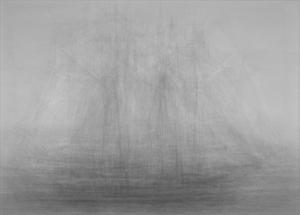
\includegraphics[height=3in]{set1grayscale.jpg}
\caption{Part A, average grayscale image}
\end{figure}

\begin{figure}[H]
\centering
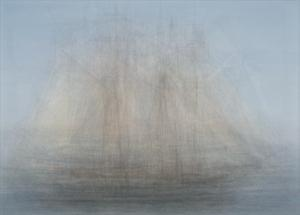
\includegraphics[height=3in]{set1color.jpg}
\caption{Part B, average color image}
\end{figure}

\begin{figure}[H]
\centering
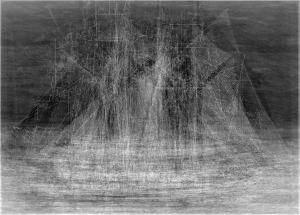
\includegraphics[height=3in]{set1grayscaleStndDev.jpg}
\caption{Part C, standard deviation image}
\end{figure}

\subsection*{set2 results}

Here are the images that resulting from running the script where the setname variable was set to $set2$. 

\begin{figure}[H]
\centering
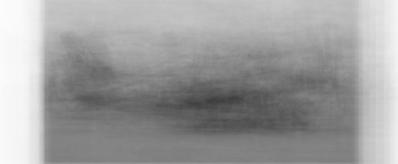
\includegraphics[height=3in]{set2grayscale.jpg}
\caption{Part A, average grayscale image}
\end{figure}

\begin{figure}[H]
\centering
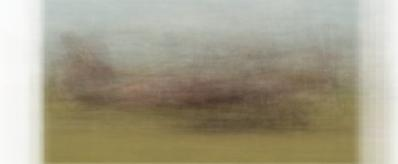
\includegraphics[height=3in]{set2color.jpg}
\caption{Part B, average color image}
\end{figure}

\begin{figure}[H]
\centering
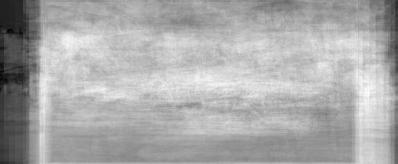
\includegraphics[height=3in]{set2grayscaleStndDev.jpg}
\caption{Part C, standard deviation image}
\end{figure}

\subsection*{Explanation of Results}

The image set $set1$ is images of sailing ships and they all look relatively similar. Therefore, the average color image and the average grayscale image looks like a sailing ship. You can definitely notice the shape of a sailing ship in the average image. In the color image it is easier to notice this due to the fact that there is more detail. The standard deviation image is darker in the background and lighter where the ship is meant to be. This could suggest that the background is often sky so it does not vary as much thus more of the varation is in the shape of the ship. 

The image set $set2$ is images of planes but there is considerable variation in background as well as type of plane. Therefore, the average color image looks vaguely like a plane but the grayscale image does not look nearly as much like a plane. The standard deviation image does not look much like a plane due to the fact that the foreground and background varies considerably between images. 

\end{document}








